\documentclass[a4paper]{article}
\usepackage[spanish]{babel}
\usepackage[utf8]{inputenc}
\usepackage{fancyhdr}
\usepackage{charter} % tipografia
%\usepackage{graphicx}
\usepackage{bytefield}
\usepackage[pdftex]{graphicx}
\usepackage{bm} % bold font in math mode
\usepackage{sidecap}
\usepackage{caption}
\usepackage{subcaption}
\usepackage{booktabs}
\usepackage{makeidx}
\usepackage{float}
\usepackage{amsmath, amsthm, amssymb}
\newtheorem{theorem}{Teorema}
\newtheorem{customthm}{Teorema}
\newtheorem{corollary}{Corolario}[theorem]
\newtheorem{proposition}[theorem]{Proposición}
\newtheorem{innercustomlemma}{Lemma}
\newenvironment{customlemma}[1]
  {\renewcommand\theinnercustomlemma{#1}\innercustomlemma}
  {\endinnercustomlemma}
\usepackage{amsfonts}
\usepackage{sectsty}
\usepackage{wrapfig}
\usepackage{listings}
\usepackage{hyperref} % links
\usepackage{algorithm} %http://www.ctan.org/pkg/algorithms
\usepackage{algorithmic}
\usepackage[usenames,dvipsnames]{xcolor}
\usepackage{pgfplots}
\usepackage{tabularx} % tablas copadas
% \usepackage{pgfplotstable}
% custom
\usepackage{color} % para snipets de codigo coloreados
\usepackage{fancybox} % para el sbox de los snipets de codigo
\definecolor{litegrey}{gray}{0.94}
% \newenvironment{sidebar}{%
% \begin{Sbox}\begin{minipage}{.85\textwidth}}%
% {\end{minipage}\end{Sbox}%
% \begin{center}\setlength{\fboxsep}{6pt}%
% \shadowbox{\TheSbox}\end{center}}
% \newenvironment{warning}{%
% \begin{Sbox}\begin{minipage}{.85\textwidth}\sffamily\lite\small\RaggedRight}%
% {\end{minipage}\end{Sbox}%
% \begin{center}\setlength{\fboxsep}{6pt}%
% \colorbox{litegrey}{\TheSbox}\end{center}}

%\newenvironment{codesnippet}{%
%\begin{Sbox}\begin{minipage}{\linewidth-2\fboxsep-2\fboxrule-4pt}\sffamily\small}%
%{\end{minipage}\end{Sbox}%
%\begin{center}%
%\colorbox{litegrey}{\TheSbox}\end{center}}

% \newenvironment{codesnippet}{\VerbatimEnvironment%
%   \noindent
%   %{\columnwidth-\leftmargin-\rightmargin-2\fboxsep-2\fboxrule-4pt}
%   \begin{Sbox}
%   \begin{minipage}{\linewidth-2\fboxsep-2\fboxrule-4pt}
%   \begin{Verbatim}
% }{%
%   \end{Verbatim}
%   \end{minipage}
%   \end{Sbox}%
%   \colorbox{litegrey}{\TheSbox}
% }

\newenvironment{codesnippet}{%
  \noindent
  %      {\columnwidth-\leftmargin-\rightmargin-2\fboxsep-2\fboxrule-4pt}
  \begin{Sbox}
  \begin{minipage}{\linewidth}
  \begin{lstlisting}
}{
  \end{lstlisting}
  \end{minipage}
  \end{Sbox}%
  \colorbox{litegrey}{\TheSbox}
}

\usepackage{fancyhdr}
\pagestyle{fancy}
%\renewcommand{\chaptermark}[1]{\markboth{#1}{}}
\renewcommand{\sectionmark}[1]{\markright{\thesection\ - #1}}
\fancyhf{}
\fancyhead[LO]{Sección \rightmark} % \thesection\
\fancyfoot[LO]{\small{Iv\'an Arcuschin, Mart\'in Jedwabny, Jos\'e Massigoge, Iv\'an Pondal}}
\fancyfoot[RO]{\thepage}
\renewcommand{\headrulewidth}{0.5pt}
\renewcommand{\footrulewidth}{0.5pt}
\setlength{\hoffset}{-0.8in}
\setlength{\textwidth}{16cm}
%\setlength{\hoffset}{-1.1cm}
%\setlength{\textwidth}{16cm}
\setlength{\headsep}{0.5cm}
\setlength{\textheight}{25cm}
\setlength{\voffset}{-0.7in}
\setlength{\headwidth}{\textwidth}
\setlength{\headheight}{13.1pt}
\renewcommand{\baselinestretch}{1.1} % line spacing

% -------------------- COMANDOS ESPECIALES ------------------------------

\newcommand{\calcular}[2]{\pgfmathtruncatemacro{#1}{#2}}

\pgfplotsset{
  filter params/.style n args={4}{
      x filter/.code={
          \edef\tempa{\thisrow{#1}}
          \edef\tempb{#2}
          \edef\tempc{\thisrow{#3}}
          \edef\tempd{#4}
          \ifx\tempa\tempb
            \ifx\tempc\tempd
            \else
              \def\pgfmathresult{inf}
            \fi
          \else
            \def\pgfmathresult{inf}
          \fi
      }
  }
}

\newcommand{\graficarDatos}[6]{
  \begin{tikzpicture}
  \begin{axis}[
      title={#1},
      xlabel={#2},
      ylabel={#3},
      scaled x ticks=false,
      scaled y ticks=false,
      scale=0.5
  ]
  \addplot[only marks, color=black] table[x=#4,y=#5]{#6};
  \end{axis}
  \end{tikzpicture}
}

\newcommand{\graficarDatosPlus}[7]{
  \begin{tikzpicture}
  \begin{axis}[
      title={#1},
      xlabel={#2},
      ylabel={#3},
      scaled x ticks=false,
      scaled y ticks=false,
      width=0.6\textwidth,
      #7
  ]
  \addplot[only marks, color=black] table[x=#4,y=#5]{#6};
  \end{axis}
  \end{tikzpicture}
}

\makeatletter
\pgfplotsset{
    groupplot xlabel/.initial={},
    every groupplot x label/.style={
        at={($({group c1r\pgfplots@group@rows.west}|-{group c1r\pgfplots@group@rows.outer south})!0.5!({group c\pgfplots@group@columns r\pgfplots@group@rows.east}|-{group c\pgfplots@group@columns r\pgfplots@group@rows.outer south})$)},
        anchor=north,
    },
    groupplot ylabel/.initial={},
    every groupplot y label/.style={
            rotate=90,
        at={($({group c1r1.north}-|{group c1r1.outer
west})!0.5!({group c1r\pgfplots@group@rows.south}-|{group c1r\pgfplots@group@rows.outer west})$)},
        anchor=south
    },
    execute at end groupplot/.code={%
      \node [/pgfplots/every groupplot x label]
{\pgfkeysvalueof{/pgfplots/groupplot xlabel}};
      \node [/pgfplots/every groupplot y label]
{\pgfkeysvalueof{/pgfplots/groupplot ylabel}};
    },
    group/only outer labels/.style =
{
group/every plot/.code = {%
    \ifnum\pgfplots@group@current@row=\pgfplots@group@rows\else%
        \pgfkeys{xticklabels = {}, xlabel = {}}\fi%
    \ifnum\pgfplots@group@current@column=1\else%
        \pgfkeys{yticklabels = {}, ylabel = {}}\fi%
}
}
}

\def\endpgfplots@environment@groupplot{%
    \endpgfplots@environment@opt%
    \pgfkeys{/pgfplots/execute at end groupplot}%
    \endgroup%
}
\makeatother

\newcommand{\barGraphExp}[2]{
    \begin{tikzpicture}
    \begin{axis}[
        xlabel={Implementación},
    	ylabel={Tiempo de ejecución (clocks)},
        legend style={at={(1.4,1.0)}},
        ybar,
        scaled ticks=false,
        width=0.5\textwidth,
        height=0.5\textwidth,
        tickpos=left,
        xtick=\empty,
        ytick align=inside,
        xtick align=inside,
    	enlargelimits=0.05,
        bar width=16,
    ]
    % How to process each item:
    \renewcommand*{\do}[1]{\addplot+[color=black] table[x=n, y=##1]{datos/datos_blur.dat};}
    % Process list:
    \docsvlist{#2}
    \legend{#2}
    \end{axis}
    \end{tikzpicture}
}

\newcommand{\graficarDatosExp}[6]{
  \begin{tikzpicture}
  \begin{axis}[
      title={#1},
      xlabel={#2},
      ylabel={#3},
      scaled x ticks=false,
      scaled y ticks=false,
      enlargelimits=0.05,
      width=0.5\textwidth,
      height=0.5\textwidth
  ]
  \addplot[color=black] table[x=#5,y=#6]{#4};
  % \renewcommand*{\do}[1]{\addplot table[x=#5,y=##1]{#4};}
  % %     % Process list:
  % \docsvlist{#6}
  % \legend{#6}
  \end{axis}
  \end{tikzpicture}
}

% ------------------------------------------------------------------------

% \setcounter{secnumdepth}{2}
\usepackage{underscore}
\usepackage{kbordermatrix}% Matrix column labels
\usetikzlibrary{arrows,shapes}
\usepackage{tkz-graph}
\usepackage{caratula}
\usepackage{url}
\lstset{
    language=C++,
    basicstyle=\ttfamily,
    keywordstyle=\color{blue}\ttfamily,
    stringstyle=\color{red}\ttfamily,
    commentstyle=\color{ForestGreen}\ttfamily,
    morecomment=[l][\color{magenta}]{\#},
    literate={á}{{\'a}}1 {ó}{{\'o}}1 {é}{{\'e}}1 {í}{{\'i}}1 {ú}{{\'u}}1 {Á}{{\'A}}1 {Í}{{\'I}}1 {É}{{\'E}}1 {Ú}{{\'U}}1 {Ó}{{\'O}}1 {\ \ }{{\ }}1,
	breaklines=true,
	tabsize=2
}

\DeclareUnicodeCharacter{2212}{-}

% *********************** %
\usepackage{tikz}
\usetikzlibrary{graphs}
\usetikzlibrary{calc}
\usetikzlibrary{arrows}
\usetikzlibrary{matrix}
% Otros
\usepackage{arrayjobx}
\usepackage{enumitem}
\usepackage{multicol}
\usepackage{natbib}
\usepackage{etoolbox}
\usepackage{listingsutf8}
\lstset{inputencoding=utf8/latin1}
\usepackage{fancyvrb}
\usepackage{pgfplotstable}
\usepackage{float}
\newcommand{\subscript}[2]{$#1 _ #2$}


% ******************************************************** %
\begin{document}
\thispagestyle{empty}
\materia{Métodos Numéricos}
\submateria{Segundo Cuatrimestre de 2015}
\titulo{Trabajo Práctico III}
%\subtitulo{Grupo: }
\integrante{Iv\'an Arcuschin}{678/13}{iarcuschin@gmail.com}
\integrante{Mart\'in Jedwabny}{885/13}{martiniedva@gmail.com}
\integrante{Jos\'e Massigoge}{954/12}{jmmassigoge@gmail.com}
\integrante{Iv\'an Pondal}{078/14}{ivan.pondal@gmail.com}
\maketitle
% no footer on the first page
\thispagestyle{empty}
\newpage

\tableofcontents

\newpage
\section{Introducción}
% El objetivo principal de este Trabajo Práctico es estudiar, implementar y analizar
 métodos de Interpolación para generar Videos con \textit{slow motion}.

Comenzaremos haciendo una breve introducción a los distintos métodos de Interpolación,
para luego explicar cual es el modelo que subyace en cada uno:
\begin{itemize}
    \item Interpolación por Vecinos.
    \item Interpolación Fragmentaria Lineal.
    \item Interpolación por Splines.
    \item Interpolación por Splines (bloques de tamaño fijo).
\end{itemize}

Una vez finalizada la parte del Modelo, pasaremos a describir la Implementación de los
diferentes métodos presentados, realizadas en \texttt{C++}.

Ya llegando al final, pasaremos a presentar la Experimentación realizada, a la vez
que iremos analizando y discutiendo los resultados obtenidos.

Los experimentos realizados pueden dividirse en dos categorías. La primera, relacionada
con el costo temporal y la correctitud de los diversos algoritmos utilizados:
\begin{itemize}
    \item Funcionamiento de los métodos implementados al tratar de interpolar diferentes
        familias de funciones.
    \item Comparación de tiempos de ejecución entre los distintos métodos.
    \item Determinación del tamaño de bloque del método Interpolación por Splines.
\end{itemize}

La segunda, relacionada con el aspecto cualitativo de los métodos:
\begin{itemize}
    \item Comparación del \textit{Error Cuadrático Medio} y \textit{Peak to Signal Noise Rate} entre
        los distintos métodos.
    \item Análisis del fenómeno de Artifacts.
\end{itemize}

Para finalizar, cerraremos el presente informe con una conclusión, en la cual
discutiremos acerca de los métodos vistos, así como de la experimentación realizada.
También, contaremos las dificultades encontradas al realizar el Trabajo Práctico,
las posibles continuaciones que se podrían realizar, y si los objetivos planteados
fueron alcanzados.


\newpage
\section{Modelo}
\subsection{Video}

Definiremos un modelo para los videos con el cual sea fácil de trabajar a la hora de realizar
el \textit{slow motion}.
Dado un video, definiremos:
\begin{itemize}
    \item $w$ el ancho en píxeles de cada frame.
    \item $h$ el ancho en píxeles de cada frame.
    \item $f_i$ el $i$-ésimo frame, con $0< i < k$, donde k es la cantidad de frames totales.
    \item $p(x,y,f_i)$, con $0 < x < w$, $0< y < h$, el píxel en la posición $(x,y)$ del frame $f_i$.
\end{itemize}

Luego, si tomamos $p(x,y,f_i)$ y $p(x,y,f_{i+1})$ querremos agregar una cierta cantidad
de píxeles entre ambos, de forma que haya una transición del primero al segundo y
se produzca el \textit{slow motion}.

Para elegir que valores agregar entre los píxeles, utilizaremos diferentes métodos
de interpolación.
\begin{itemize}
    \item \textit{Vecinos}: Consiste en rellenar los nuevos frames replicando los
        valores de los píxeles del frame original que se encuentra más cerca.
    \item \textit{Interpolación Lineal}: Consiste en rellenar los píxeles utilizando
        interpolaciones lineales entre píxeles de frames originales consecutivos.
    \item \textit{Interpolación por Splines}: Consiste en rellenar los píxeles utilizando
        Splines entre píxeles de frames originales consecutivos. En este método,
        utilizaremos la información provista por todos los frames del video,
        y generaremos $k-1$ funciones, cada una de a lo sumo grado cúbico.
    \item \textit{Interpolación por Splines con tamaño de bloque variante}:
        Simliar al anterior, pero con la posibilidad de variar la cantidad de frames
        tomados en cuenta al generar las funciones.
\end{itemize}

En las siguientes secciones explicaremos con mayor detalle cada uno de los métodos.

\subsection{Vecinos}\label{Vecinos}
En este método, eligiremos para cada nuevo píxel el valor del frame original que se encuentre
más cercano.
Si definimos $c$ como la cantidad de frames a agregar entre cada par original, y
$g_0, \dots, g_{c-1}$ los nuevos frames. Tenemos que:
\begin{equation*}
    \begin{aligned}
        p(x,y,f_{i}) &= p(x,y,f_{i})\\
        p(x,y,g_{0}) &= p(x,y,f_{i})\\
        \vdots\\
        p(x,y,g_{c/2-1}) &= p(x,y,f_{i})\\
        p(x,y,g_{c/2}) &= p(x,y,f_{i+1})\\
        \vdots\\
        p(x,y,g_{c-1}) &= p(x,y,f_{i+1})\\
        p(x,y,f_{i+1}) &= p(x,y,f_{i+1})
    \end{aligned}
\end{equation*}

\subsection{Interpolación Lineal}\label{Lineal}
En este método, buscaremos interpolar los píxeles de frames contiguos con una función
lineal. Para ello, construiremos un Polinomio Interpolante de grado 1 utilizando
\textit{diferencias divididas}, ya que ofrece una construcción más sencilla que al seguir
el método de Lagrange.

Luego, si llamamos $f$ a la función (desconocida excepto en los puntos $x_j$), definimos:
\begin{itemize}
    \item Diferencia dividida de orden cero en $x_j$:
        \begin{equation*}
            f[x_j] = f(x_j)
        \end{equation*}
    \item Diferencia dividida de orden uno en $x_j$, $x_{j+1}$:
        \begin{equation*}
            f[x_j,x_{j+1}]= \frac{f[x_{j+1}] - f[x_j]}{x_{j+1} - x_j} = \frac{f(x_{j+1}) - f(x_j)}{x_{j+1} - x_j}
        \end{equation*}
    \item Polinomio Interpolante de grado 1 para $x_j$, $x_{j+1}$:
        \begin{equation*}
            P_1(x) = f[x_j] + f[x_j,x_{j+1}](x-x_j) = f(x_j) + \frac{f(x_{j+1}) - f(x_j)}{x_{j+1} - x_j}*(x-x_j)
        \end{equation*}
\end{itemize}

\subsection{Interpolación por Splines}\label{Splines}

\subsection{Interpolación por Splines con tamaño de bloque variante}\label{MultiSplines}


\newpage
\section{Implementación}
\subsection{Interpolación por vecinos}

Este método consiste en reemplazar los cuadros intermedios a ser rellenados por el cuadro original mas cercano en el tiempo.
Es decir, dados los cuadros del video sin camara lenta, generamos otro video en camara lenta copiando los cuadros originales de la siguiente manera:

% \begin{bytefield}{16}
% \wordbox{1}{A 16-bit field} \\
% \bitbox{8}{8 bits} & \bitbox{8}{8 more bits} \\
% \wordbox{2}{A 32-bit field. Note that text wraps within the box.}
% \end{bytefield}

Sean Frame1 y Frame2 dos cuadros consecutivos del video original:

\begin{bytefield}{8}
\bitbox{4}{Frame1} & \bitbox{4}{Frame2}
\end{bytefield}

Si queremos ahora 6 cuadros entre cada 2 del archivo original lo transformamos a:

\begin{bytefield}{32}
\bitbox{4}{Frame1} & \bitbox{4}{Frame1} & \bitbox{4}{Frame1} & \bitbox{4}{Frame1} & \bitbox{4}{Frame2} & \bitbox{4}{Frame2} & \bitbox{4}{Frame2} & \bitbox{4}{Frame2}
\end{bytefield}

El pseudocódigo sería el siguiente:

\begin{lstlisting}
Sean W,H,I el ancho, alto y la cantidad de frames del video original
Sea video[W][H][I] el triple vector de numeros enteros que representa el video original
Sea K la cantidad de frames que queremos agregar entre cuadro y cuadro

Crear un triple vector de enteros new_video[W][H][I+(I-1)*K]
Para w = 0 hasta W-1 hacer
	Para h = 0 hasta H-1 hacer
		Para i = 0 hasta I-2 hacer
			Para j = 0 hasta K/2 hacer
				new_video[w][h].push_back(video[w][h][i])
			Fin para
			Para j = (K/2)+1 hasta K hacer
				new_video[w][h].push_back(video[w][h][i+1])
			Fin para
		Fin para
		new_video[w][h].push_back(video[w][h][I-1])
	Fin para
Fin para
Devolver new_video
\end{lstlisting}

\subsection{Interpolación lineal}

En este caso, usamos el polinomio interpolador de Lagrange entre cada par de puntos/pixeles consecutivos para aproximar los valores intermedios que irían en el video de camara lenta. Esto genera una función lineal para los pixeles consecutivos en la misma posición.

Por ejemplo, sean dos pixeles con valores 1 y 4:

\begin{bytefield}{8}
\bitbox{4}{1} & \bitbox{4}{4}
\end{bytefield}

Si queremos un video en camara lenta con 5 cuadros intermedios por cada 2 del original, estos se replicarán de la siguiente forma:

\begin{bytefield}{28}
\bitbox{4}{1} & \bitbox{4}{1.5} & \bitbox{4}{2} & \bitbox{4}{2.5} & \bitbox{4}{3} & \bitbox{4}{3.5} & \bitbox{4}{4}
\end{bytefield}

El procedimiento es el siguiente:

\begin{lstlisting}
Sean W,H,I el ancho, alto y la cantidad de frames del video original
Sea video[W][H][I] el triple vector de numeros enteros que representa el video original
Sea K la cantidad de frames que queremos agregar entre cuadro y cuadro

Crear un triple vector de enteros new_video[W][H][I+(I-1)*K]
Para w = 0 hasta W-1 hacer
	Para h = 0 hasta H-1 hacer
		Para i = 0 hasta I-2 hacer
			coef_cero = video[w][h][i]
			coef_uno = (video[w][h][i+1] - video[w][h][i]) / (K+1);
			Para k = 0 hasta K hacer
				pixel = coef_cero + coef_uno*k;
				Si (pixel < 0) pixel = 0
				Si (pixel > 255) pixel = 255
				new_video.push_back(pixel)
		Fin para
		new_video.push_back(video[w][h][I-1])
	Fin para
Fin para
Devolver new_video
\end{lstlisting}

\subsection{Interpolación por Splines}

En este método aplicamos la técnica de Splines. Esta consiste en generar un sistema de ecuaciones para encontrar una función por partes que interpole cada par de puntos con polinomios de forma que la curva resultante sea continua y dos veces derivable. Como el sistema es tridiagonal, podemos aprovechar para guardar los valores de la matriz de forma más eficiente. El pseudocódigo es el siguiente:

\begin{lstlisting}
Sean W,H,I el ancho, alto y la cantidad de frames del video original
Sea video[W][H][I] el triple vector de numeros enteros que representa el video original
Sea K la cantidad de frames que queremos agregar entre cuadro y cuadro

Crear un triple vector de enteros new_video[W][H][I+(I-1)*K]
Para w = 0 hasta W-1 hacer
	Para h = 0 hasta H-1 hacer
		new_video[w][h] = GenerarSpline(video[w][h])
	Fin para
Fin para
Devolver new_video

GenerarSpline(y[n]):
	Crear un vector de enteros valores[I+(I-1)*K]
	Crear doble vector de enteros sistema[n][2]
	sistema[0] = {1,0}
	Para j = 1 hasta n-2 hacer
		sistema[j] = {1, 4}
	Fin para
	sistema[n-1] = {0,1}
	// Factorización LU
	Para j = 1 hasta n-2 hacer
		coef = sistema[i + 1][0]/sistema[i][1];
		sistema[i + 1][0] = coef
		sistema[i + 1][1] -= coef
	Fin para
	Crear vectores x[n], a[n], b[n], c[n], d[n]
	a = y
	Para i = 1 hasta n-2 hacer
		x[i] = 3*(a[i + 1] - 2*a[i] + a[i - 1]);
		x[i] -= x[i - 1]*sistema[i][0];
	Fin para
	// Resuelvo triangular superior (Uc = x)
	Para i = n - 2 hasta 1 hacer
		c[i] = x[i];
		c[i] -= c[i + 1];
		c[i] /= sistema[i][1];
	Fin para
	// Calculo mis coeficientes "b" y "d"
	Para i = 0 hasta n-2 hacer
		b[i] = a[i + 1] - a[i] - (2*c[i] + c[i + 1])/3;
		d[i] = (c[i + 1] - c[i])/3;
	Fin para
	//Calculo los pixeles resultantes con el Spline
	Para i = 0 hasta n-1 hacer
		Para j = 0 hasta K hacer
			dif = j/(K+1)
			val = a[i] + b[i]*(dif) + c[i]*(dif)*(dif) + d[i]*(dif)*(dif)*(dif)
			valores.push_back(val)
		Fin para
	Fin para
	valores.push_back(y[n-1])
	Devolver valores
\end{lstlisting}

\subsection{Interpolación por Splines de a bloques}

A diferencia del método anterior, en este caso vamos a querer aplicar la técnica de Splines a bloques de pixeles de tamaño fijo. Es decir, para una misma posición del video, en vez de utilizar todos los valores del pixel a través del tiempo, generamos splines entre particiones de la misma longitud. El procedimiento es:

\begin{lstlisting}
Sean W,H,I el ancho, alto y la cantidad de frames del video original
Sea video[W][H][I] el triple vector de numeros enteros que representa el video original
Sea K la cantidad de frames que queremos agregar entre cuadro y cuadro
Sea T el tamano de bloque de los Splines
Observacion: reutilizamos el metodo GenerarSpline(y) de los Splines normales
Observacion: asumimos que I es divisible por T para simplificar este pseudocodigo

Crear un triple vector de enteros new_video[W][H][I+(I-1)*K]
Para w = 0 hasta W-1 hacer
	Para h = 0 hasta H-1 hacer
		Para t = 0 hasta T-1 hacer
			Crear subarreglo aux[T] = video[w][h][T*t..T*(t+1)-1]
			Crear arreglo bloque[T] = GenerarSpline(aux)
			Pushear a new_video[w][h] todos los valores de 'bloque'
		Fin para
	Fin para
Fin para
Devolver new_video
\end{lstlisting}

\newpage
\section{Experimentación}
En esta sección, se detallan los diferentes experimentos que realizamos para medir el funcionamiento, la eficiencia y calidad de resultados, tanto de forma cuantitativa como cualitativa, de los métodos implementados.

Para lograr tal fin realizamos los siguientes tipos de experimentos:
\begin{itemize}
  \item Funcionamiento de los métodos implementados: Mostraremos que los métodos
        de interpolación funcionan correctamente comparandolos contra diferentes
        familias de funciones. A su vez, basandonos en las precisiones obtenidas,
        determinaremos el tamaño de bloque óptimo para el método Interpolación por Splines.
  \item Medición del ECM y PSNR de los métodos: Compararemos los errores obtenidos
        en varias instancias de pruebas para los distintos métodos.
  \item Medición de los tiempos de ejecución de los métodos: Compararemos los
        tiempos de ejecución utilizando los distintos métodos.
  \item Análisis cualitativos de los métodos, fenómeno de artifacts: Buscaremos
        reconocer defectos de interpolación en los videos generados.
\end{itemize}

Los videos utilizados para los diversos experimentos, fueron los siguientes:

\begin{itemize}
  \item \textbf{Video 1 - Skate}: 426x240, cantidad de cuadros originales: 151 , fps: 30, duracion: 5s.
  \item \textbf{Video 2 - Messi}: 426x240, cantidad de cuadros originales: 151, fps: 30, duracion: 5s.
  \item \textbf{Video 3 - Amanecer}: 426x240, cantidad de cuadros originales: 151, fps: 30, duracion: 5s.
\end{itemize}

Es importante mencionar que cada video representa una clase de video distinto, en donde el Video 1 contiene movimientos bruscos, el Video 2 cambios de camara, y el Video 3 movimientos suaves.

El motivo de estas elecciones se debe a la busqueda de diversos \textit{artifacts} a partir de las caracteristicas de cada clase.

\subsection{Detalles generales de la experimentación}

\begin{itemize}
    \item En los experimentos que se utilizaron números aleatorios, se generaron utilizando la función \textit{rand}, provista por la librería \texttt{stdlib.h}.
    \item La semilla para los números aleatorios se seteo utilizando el método \textit{srand(time(NULL))}, para evitar repeticiones de números en diferentes corridas.
    \item Las instancias de prueba fueron generadas con los archivos provistos por la cátedra. Adicionalmente, hicimos nuestras propias instancias emulando diferentes funciones (por ejemplo una función constante, lineal y cuadrática) para realizar el control de calidad de los métodos.
    \item Para medir los tiempos utilizamos la librería \textit{chrono} y medimos los resultados en nanosegundos.
    \item A su vez, utilizamos el nivel de optimización \textit{O2} de \textit{C++} a la hora de compilar el código.
    \item Todos los tests fueron corridos en la misma máquina bajo las mismas condiciones.
\end{itemize}


\subsection{Funcionamiento de los métodos implementados}\label{exp_funcionamiento}
En este experimento nuestro objetivo fue asegurarnos el correcto funcionamiento de nuestra implementación de la interpolación fragmentaria lineal, interpolación por splines, e interpolación por splines con tamaño de bloque fijo, tomando bloques de 2, 4, 8, 16, 32 y 64 cuadros.

Con este fin, realizamos una serie de tests que muestran el correcto funcionamiento de cada método para distintas familias de funciones:
\begin{itemize}
  \item Función constante.
  \item Función lineal.
  \item Función cuadrática.
  \item Función cúbica.
\end{itemize}

Luego, cada método de interpolación fue testeado contra cada una de las familias de funciones mencionadas de la siguiente forma:
\begin{itemize}
  \item Dada una familia de funciones, se generan aleatoriamente los coeficientes necesarios para definir una función de esa familia, i.e.: para una constante se genera solo el coeficiente independiente, mientras que para una cuadrática se generan 3 coeficientes.
    \item Una vez generada la función, se la evalua en un rango de valores para obtener un array de valores esperados.
    \item Luego, a partir del array de valores esperados se construye otro array quitandole elementos a intervalos fijos.
        Este nuevo array será el utilizado para realizar la interpolación, y lo que testearemos es la aproximación de  la
        interpolación a los elementos que quitamos.
    \item Una vez que tenemos la interpolación con cualquiera de los métodos mencionados, basta recorrer los elementos del array de valores esperados a la vez que evaluamos la interpolación obtenida.
        Para cada par de valores: esperado e interpolado, querremos ver que la diferencia absoluta es menor que un epsilon/cota de precision que
        definiremos dependiendo del método utilizado y la función a interpolar.
\end{itemize}

Es importante mencionar algunas carácterísticas de las instancias utilizadas:
\begin{itemize}
    \item Cantidad de puntos generados con la función(tamaño del array de valores esperados): 100
    \item Cantidad de puntos a interpolar: 50.
    \item Todos los coeficientes generados aleatoriamente están en el rango $[1,10]$,
        para evitar que las funciones generadas crezcan de forma desmedida.
\end{itemize}

Luego, se obtuvieron las siguientes cotas de precisión para los distintos métodos y funciones:

\begin{table}[H]
    \begin{tabular}{| c | c | c | c | c |}
    \hline
    {} & F. Constante & F. Lineal & F. Cuadrática & F. Cúbica \\ \hline
    Interpolación por Vecinos & 0.0001 & 10 & 1000 & 100000 \\
    Interpolación Fragmentaria Lineal & 0.0001 & 0.0001 & 10 & 1000 \\
    Interpolación por Splines (bloques tamaño 2) & 0.0001 & 0.0001 & 10 & 1000 \\
    Interpolación por Splines (bloques tamaño 4) & 0.0001 & 0.0001 & 5 & 500 \\
    Interpolación por Splines (bloques tamaño 8) & 0.0001 & 0.0001 & 1 & 200 \\
    Interpolación por Splines (bloques tamaño 16) & 0.0001 & 0.0001 & 1 & 200 \\
    Interpolación por Splines (bloques tamaño 32) & 0.0001 & 0.0001 & 1 & 200 \\
    Interpolación por Splines (bloques tamaño 64) & 0.0001 & 0.0001 & 1 & 200 \\
    Interpolación por Splines (1 solo bloque) & 0.0001 & 0.0001 & 1 & 200 \\
    \hline
    \end{tabular}
\end{table}

Analizando dichas cotas vemos que:
\begin{itemize}
    \item La Interpolación por Vecinos resulta razonable solo para funciones con muy
        poca variación (derivada a lo sumo constante). Esto se ve claramente en la
        cota de presición al interpolar una función Cuadrática.
    \item La Interpolación Fragmentaria Lineal es sustancialmente mejor que por Vecinos,
        y devuelve resultados razonables para funciones a lo sumo Cuadráticas.
    \item La Interpolación por Splines utilizando solo 2 puntos para cada bloque es
        equivalente a interpolar utilizando funciones lineales, y queda evidenciado al
        tener las mismas cotas de precisión.
    \item A partir de los tamaños de bloque 4 a 16, la Interpolación por Splines realiza
        una mejora ``asintótica'' de su cota de precisión.
    \item Entre los tamaños de bloque 16 a 64, no se notó una mejora significativa en la cota
        de precisión de la Interpolación por Splines.
    \item Al realizar Interpolación por Splines \textit{standard} (1 solo bloque),
        vemos que su cota de precisión concuerda con las cotas a las cuales ``convergen''
        los métodos de Interpolación por Splines con bloque de tamaño fijo. Es por esta razón
        que para los experimentos cualitativos, utilizaremos solamente la Interpolación
        por Splines \textit{standard}, y no la de tamaño de bloques fijo.
\end{itemize}

\subsection{Medición de los tiempos de ejecución de los métodos}
A partir de la implementaciones descriptas en la Sección \ref{Implementacion},
podemos inferir una complejidad temporal para cada método.

Sea $w$ la cantidad de filas de píxeles en cada imagen, $h$ la cantidad de
columnas, $i$ la cantidad de cuadros originales y sea $k$ la cantidad de
cuadros a agregar entre los originales:

Todos los metodos implementados tienen la misma complejidad temporal que es
 $\Theta(w*h*i*k*)$. Esta conclusion surge del hecho de que, en todos los casos,
 tenemos 4 ciclos anidados, en donde el primero se ejecuta $w$ veces, el segundo
 $h$ veces, el tercero $i$ veces, y el cuarto $k$ veces.
%\begin{itemize}
%  \item Vecino mas cercano: realizamos 4 ciclos anidados, en donde el primero se ejecuta $w$ veces, el segundo $h$ veces, el tercero $i$ veces, y el cuarto $k$ veces, la complejidad temporal del mismo es $\Theta(whik)$.
%  \item Interpolacion lineal: situacion identica a la de vecinos mas cercanos, por lo tanto su complejidad temporal es de $\Theta(whik)$.
%  \item Interpolacion por Splines: en este caso realizamos primero un ciclo que se ejecuta $w$ veces, dentro de este ciclamos $h$
%  \item Interpolacion por Splines con tamaño de bloque fijo:
%\end{itemize}
\newline
\newline
Para corroborar esta hipotesis planteamos un experimento con las siguientes caracteristicas:
\begin{itemize}
  \item Utilizamos el video provisto por la catedra llamado \textit{funnybaby}, el cual tiene 44 cuadros y es de 240x320.
  \item Solo medimos la resolucion del sistema, no su creacion o los respectivos pasajes de video a texto y viceversa.
  \item Dado que $w$, $h$ y $i$ son valores fijos que no podemos cambiar, variamos el $k$.
  \item Generamos instancias para valores de $k$ entre 1 y 6.
  \item Para cada valor distinto de $k$ generamos 4 instancias, cuyos valores vamos a promediar para mitigar los posibles valores distorsionados por algun procedimiento del procesador.
\end{itemize}

Los resultamos obtenidos fueron los siguientes:

\begin{center}
    \begin{tikzpicture}
    \begin{axis}[
        title={},
        xlabel={cantidad de cuadros agregados entre originales ($k$)},
        ylabel={tiempo (nanosegundos)},
        ylabel absolute,
        ylabel style={yshift=.3cm},
        scaled x ticks=false,
        scaled y ticks=false,
        enlargelimits=0.05,
        width=0.85\textwidth,
        height=0.45\textwidth,
        legend style={at={(1.015,1)},anchor=north west},
        no markers,
        thick,
        cycle list name=exotic
    ]
    \addplot[color=green] table[x index=0,y index=1]{datos/timelineal};
    \addplot[color=red] table[x index=0,y index=1]{datos/timevecinos};
    \addplot[color=blue] table[x index=0,y index=1]{datos/timesplines};
    \legend{Lineal, Vecinos, Splines}
    \end{axis}
    \end{tikzpicture}
\end{center}

Si tomamos los tiempos que arrojó la experimentación, y los dividimos por su respectivo $k$, obtenemos el siguiente resultado:

\begin{center}
    \begin{tikzpicture}
    \begin{axis}[
        title={},
        xlabel={cantidad de cuadros agregados entre originales ($k$)},
        ylabel={tiempo (nanosegundos) / $k$},
        ylabel absolute,
        ylabel style={yshift=.3cm},
        scaled x ticks=false,
        scaled y ticks=false,
        enlargelimits=0.05,
        width=0.85\textwidth,
        height=0.45\textwidth,
        legend style={at={(1.015,1)},anchor=north west},
        no markers,
        thick,
        cycle list name=exotic
    ]
    \addplot[color=green] table[x index=0,y index=2]{datos/timelineal};
    \addplot[color=red] table[x index=0,y index=2]{datos/timevecinos};
    \addplot[color=blue] table[x index=0,y index=2]{datos/timesplines};
    \legend{Lineal, Vecinos, Splines}
    \end{axis}
    \end{tikzpicture}
\end{center}

A partir de los graficos, queda de manifiesto que los metodos tienen la misma complejidad temporal, ya que solo difieren en una constante.

\subsection{Medición del ECM y PSNR de los métodos.}\label{ECM}
Sea $F$ un frame del vídeo real (ideal) , y $\bar{F}$ el mismo frame del vídeo efectivamente construidos por alguno de los métodos. Sea $m$ la cantidad de filas de píxeles en cada imagen y $n$ la cantidad de columnas.

Definimos el Error Cuadrático Medio, \texttt{ECM}, como el real dado por:
\begin{equation}
\texttt{ECM}(F,\bar{F}) = \frac{1}{mn}\sum_{i=1}^m\sum_{j = 1}^n |F_{k_{ij}} - \bar{F}_{k_{ij}}|^2
\end{equation}

A su vez definimos \emph{Peak to Signal Noise Ratio}, \texttt{PSNR}, como el real dado por:
\begin{equation}
\texttt{PSNR}(F,\bar{F}) = 10 \log_{10}\bigg(\frac{255^2}{\texttt{ECM}(F,\bar{F})}\bigg). \label{eq:psnr}
\end{equation}

Ambas medidas nos sirven para realizar un análisis cuantitativo de la calidad de los resultados obtenidos con los distintos métodos.

En este experimento utilizamos los videos propuestos al inicio de la experimentacion, variando la cantidad de cuadros que agregamos.
Dichos videos fueron elegidos especificamente para variar la dificultad de Interpolación:
\begin{itemize}
    \item El video \textbf{Amanecer} no contiene movimientos bruscos ni cambios de cámaras
        por lo que, para cualquier método, el error debería ser en lineas generales
        menor que pare el resto de los videos.
    \item El video \textbf{Skate} contiene movimientos bruscos pero no cambios de cámaras
        por lo que, se espera un mayor error que en el video anterior. Además,
        deberíamos ver un aumento del error en los frames donde hay movimientos
        bruscos.
    \item El video \textbf{Skate} contiene movimientos bruscos y cambios de cámaras
        por lo que, se espera un mayor error que en el resto de los videos. Además,
        deberíamos ver un aumento \textit{importante} del error en los frames
        donde se produce el cambio de cámara.
\end{itemize}

A continuación, presentaremos e iremos analizando los resultados obtenidos:

\subsubsection{ECM - Agregando 1 cuadro}

\begin{figure}[H]
	\centering
	\begin{tikzpicture}
		\begin{axis}[
			title={ },
			xlabel=Frame,
			ylabel=ECM,
			width=0.8\textwidth,
			height=0.5\textwidth,
			yticklabel style={/pgf/number format/fixed},
			scaled y ticks=false,
			legend style={at={(1.015,1)},anchor=north west},
			no markers,
			thick,
            cycle list name=exotic
		]
		\addplot table[x index=0,y index=1]{../src/exp/error-sunrise-vecinos1};
        \addplot[color=blue] table[x index=0,y index=1]{../src/exp/error-sunrise-lineal1};
        \addplot[color=red] table[x index=0,y index=1]{../src/exp/error-sunrise-spline1};
		\legend{Vecinos, Lineal, Spline}
		\end{axis}
	\end{tikzpicture}
	\caption{ECM para el video \textbf{Amanecer} al agregar 1 cuadro con distintos métodos de Interpolación.}
	\label{fig:ecm_sunrise_1}
\end{figure}

\begin{figure}[H]
	\centering
	\begin{tikzpicture}
		\begin{axis}[
			title={ },
			xlabel=Frame,
			ylabel=ECM,
			width=0.8\textwidth,
			height=0.5\textwidth,
			yticklabel style={/pgf/number format/fixed},
			scaled y ticks=false,
			legend style={at={(1.015,1)},anchor=north west},
			no markers,
			thick,
			cycle list name=exotic
		]
		\addplot table[x index=0,y index=1]{../src/exp/error-skate-vecinos1};
        \addplot[color=blue] table[x index=0,y index=1]{../src/exp/error-skate-lineal1};
        \addplot[color=red] table[x index=0,y index=1]{../src/exp/error-skate-spline1};
		\legend{Vecinos, Lineal, Spline}
		\end{axis}
	\end{tikzpicture}
	\caption{ECM para el video \textbf{Skate}  al agregar 1 cuadro con distintos métodos de Interpolación.}
	\label{fig:ecm_skate_1}
\end{figure}

\begin{figure}[H]
	\centering
	\begin{tikzpicture}
		\begin{axis}[
			title={ },
			xlabel=Frame,
			ylabel=ECM,
			width=0.8\textwidth,
			height=0.5\textwidth,
			yticklabel style={/pgf/number format/fixed},
			scaled y ticks=false,
			legend style={at={(1.015,1)},anchor=north west},
			no markers,
			thick,
			cycle list name=exotic
		]
		\addplot table[x index=0,y index=1]{../src/exp/error-messi-vecinos1};
        \addplot[color=blue] table[x index=0,y index=1]{../src/exp/error-messi-lineal1};
        \addplot[color=red] table[x index=0,y index=1]{../src/exp/error-messi-spline1};
		\legend{Vecinos, Lineal, Spline}
		\end{axis}
	\end{tikzpicture}
	\caption{ECM para el video \textbf{Messi}  al agregar 1 cuadro con distintos métodos de Interpolación.}
	\label{fig:ecm_messi_1}
\end{figure}

Viendo las Figuras \ref{fig:ecm_sunrise_1}, \ref{fig:ecm_skate_1} y \ref{fig:ecm_messi_1} podemos decir que:
\begin{itemize}
    \item La Interpolación por Vecinos obtiene consistentemente un mayor error que
        el resto de los métodos.
    \item La Interpolación Fragmentaria Lineal y la Interpolación por Splines obtienen
        en general un error similar, siendo la primera ligeramente mejor.
    \item El rango de error obtenido por todos los métodos en el video \textbf{Amanecer},
        es significativamente menor que en el resto de los videos. Además, se puede ver
        que el error obtenido en ese video es en cierta forma ``regular'', lo cual
        tiene sentido ya que tiene movimientos suaves y repetitivos.
    \item El rango de error obtenido por todos los métodos en los videos \textbf{Skate} y \textbf{Messi},
        son similares, y ambos mayores al rango obtenido en el video \textbf{Amanecer}.
    \item El error obtenido en el video \textbf{Skate} es bastante irregular
        al compararlo con el video \textbf{Amanecer}, encontrandose un pico de error
        en el movimiento más brusco del video.
    \item A diferencia del caso anterior, el error obtenido en el video \textbf{Messi}
        es bastante regular, a excepción del pico de error que encontramos cuando
        ocurre el cambio de cámara, el cual es notorio para todos los métodos.
\end{itemize}

\subsubsection{PSNR - Agregando 1 cuadro}
\begin{figure}[H]
	\centering
	\begin{tikzpicture}
		\begin{axis}[
			title={ },
			xlabel=Frame,
			ylabel=PSNR,
			width=0.8\textwidth,
			height=0.5\textwidth,
			yticklabel style={/pgf/number format/fixed},
			scaled y ticks=false,
			legend style={at={(1.015,1)},anchor=north west},
			no markers,
			thick,
			cycle list name=exotic
		]
		\addplot table[x index=0,y index=2]{../src/exp/error-sunrise-vecinos1};
        \addplot[color=blue] table[x index=0,y index=2]{../src/exp/error-sunrise-lineal1};
        \addplot[color=red] table[x index=0,y index=2]{../src/exp/error-sunrise-spline1};
		\legend{Vecinos, Lineal, Spline}
		\end{axis}
	\end{tikzpicture}
	\caption{PSNR para el video \textbf{Amanecer} al agregar 1 cuadro con distintos métodos de Interpolación.}
	\label{fig:psnr_sunrise_1}
\end{figure}

\begin{figure}[H]
	\centering
	\begin{tikzpicture}
		\begin{axis}[
			title={ },
			xlabel=Frame,
			ylabel=PSNR,
			width=0.8\textwidth,
			height=0.5\textwidth,
			yticklabel style={/pgf/number format/fixed},
			scaled y ticks=false,
			legend style={at={(1.015,1)},anchor=north west},
			no markers,
			thick,
			cycle list name=exotic
		]
		\addplot table[x index=0,y index=2]{../src/exp/error-skate-vecinos1};
        \addplot[color=blue] table[x index=0,y index=2]{../src/exp/error-skate-lineal1};
        \addplot[color=red] table[x index=0,y index=2]{../src/exp/error-skate-spline1};
		\legend{Vecinos, Lineal, Spline}
		\end{axis}
	\end{tikzpicture}
	\caption{PSNR para el video \textbf{Skate} al agregar 1 cuadro con distintos métodos de Interpolación.}
	\label{fig:psnr_skate_1}
\end{figure}

\begin{figure}[H]
	\centering
	\begin{tikzpicture}
		\begin{axis}[
			title={ },
			xlabel=Frame,
			ylabel=PSNR,
			width=0.8\textwidth,
			height=0.5\textwidth,
			yticklabel style={/pgf/number format/fixed},
			scaled y ticks=false,
			legend style={at={(1.015,1)},anchor=north west},
			no markers,
			thick,
			cycle list name=exotic
		]
		\addplot table[x index=0,y index=2]{../src/exp/error-messi-vecinos1};
        \addplot[color=blue] table[x index=0,y index=2]{../src/exp/error-messi-lineal1};
        \addplot[color=red] table[x index=0,y index=2]{../src/exp/error-messi-spline1};
		\legend{Vecinos, Lineal, Spline}
		\end{axis}
	\end{tikzpicture}
	\caption{PSNR para el video \textbf{Messi} al agregar 1 cuadro con distintos métodos de Interpolación.}
	\label{fig:psnr_messi_1}
\end{figure}

Sabiendo que, mientras más grande es el \texttt{ECM} más chico es el \texttt{PSNR},
encontramos que la información provista por este último no aporta nuevos elementos
al análisis, ya que se condice con lo análizado previamente utilizando el \texttt{ECM}.

\subsubsection{ECM - Agregando 5 cuadros}

\begin{figure}[H]
	\centering
	\begin{tikzpicture}
		\begin{axis}[
			title={ },
			xlabel=Frame,
			ylabel=ECM,
			width=0.8\textwidth,
			height=0.5\textwidth,
			yticklabel style={/pgf/number format/fixed},
			scaled y ticks=false,
			legend style={at={(1.015,1)},anchor=north west},
			no markers,
			thick,
			cycle list name=exotic
		]
		\addplot table[x index=0,y index=1]{../src/exp/error-sunrise-vecinos5};
        \addplot[color=blue] table[x index=0,y index=1]{../src/exp/error-sunrise-lineal5};
        \addplot[color=red] table[x index=0,y index=1]{../src/exp/error-sunrise-spline5};
		\legend{Vecinos, Lineal, Spline}
		\end{axis}
	\end{tikzpicture}
	\caption{ECM para el video \textbf{Amanecer} al agregar 5 cuadros con distintos métodos de Interpolación.}
	\label{fig:ecm_sunrise_5}
\end{figure}

\begin{figure}[H]
	\centering
	\begin{tikzpicture}
		\begin{axis}[
			title={ },
			xlabel=Frame,
			ylabel=ECM,
			width=0.8\textwidth,
			height=0.5\textwidth,
			yticklabel style={/pgf/number format/fixed},
			scaled y ticks=false,
			legend style={at={(1.015,1)},anchor=north west},
			no markers,
			thick,
			cycle list name=exotic
		]
		\addplot table[x index=0,y index=1]{../src/exp/error-skate-vecinos5};
        \addplot[color=blue] table[x index=0,y index=1]{../src/exp/error-skate-lineal5};
        \addplot[color=red] table[x index=0,y index=1]{../src/exp/error-skate-spline5};
		\legend{Vecinos, Lineal, Spline}
		\end{axis}
	\end{tikzpicture}
	\caption{ECM para el video \textbf{Skate} al agregar 5 cuadros con distintos métodos de Interpolación.}
	\label{fig:ecm_skate_5}
\end{figure}

\begin{figure}[H]
	\centering
	\begin{tikzpicture}
		\begin{axis}[
			title={ },
			xlabel=Frame,
			ylabel=ECM,
			width=0.8\textwidth,
			height=0.5\textwidth,
			yticklabel style={/pgf/number format/fixed},
			scaled y ticks=false,
			legend style={at={(1.015,1)},anchor=north west},
			no markers,
			thick,
			cycle list name=exotic
		]
		\addplot table[x index=0,y index=1]{../src/exp/error-messi-vecinos5};
        \addplot[color=blue] table[x index=0,y index=1]{../src/exp/error-messi-lineal5};
        \addplot[color=red] table[x index=0,y index=1]{../src/exp/error-messi-spline5};
		\legend{Vecinos, Lineal, Spline}
		\end{axis}
	\end{tikzpicture}
	\caption{ECM para el video \textbf{Messi} al agregar 5 cuadros con distintos métodos de Interpolación.}
	\label{fig:ecm_messi_5}
\end{figure}

Viendo las Figuras \ref{fig:ecm_sunrise_5}, \ref{fig:ecm_skate_5} y \ref{fig:ecm_messi_5} podemos decir que:
\begin{itemize}
    \item El comportamiento general de los métodos para cada video no varió con respecto
        al escenario en el cual agregabamos 1 cuadro. Los análisis de movimiento brusco y
        cambios de cámaras se reafirman.
    \item En lineas generales, y en todos los videos, el error se incrementó con respecto al
        escenario en el cual agregabamos 1 cuadro, a excepción del método de Interpolación
        por Vecinos, que mantiene su rango de error.
\end{itemize}

\subsubsection{PSNR - Agregando 5 cuadros}
\begin{figure}[H]
	\centering
	\begin{tikzpicture}
		\begin{axis}[
			title={ },
			xlabel=Frame,
			ylabel=PSNR,
			width=0.8\textwidth,
			height=0.5\textwidth,
			yticklabel style={/pgf/number format/fixed},
			scaled y ticks=false,
			legend style={at={(1.015,1)},anchor=north west},
			no markers,
			thick,
			cycle list name=exotic
		]
		\addplot table[x index=0,y index=2]{../src/exp/error-sunrise-vecinos5};
        \addplot[color=blue] table[x index=0,y index=2]{../src/exp/error-sunrise-lineal5};
        \addplot[color=red] table[x index=0,y index=2]{../src/exp/error-sunrise-spline5};
		\legend{Vecinos, Lineal, Spline}
		\end{axis}
	\end{tikzpicture}
	\caption{PSNR para el video \textbf{Amanecer} al agregar 5 cuadros con distintos métodos de Interpolación.}
	\label{fig:psnr_sunrise_5}
\end{figure}

\begin{figure}[H]
	\centering
	\begin{tikzpicture}
		\begin{axis}[
			title={ },
			xlabel=Frame,
			ylabel=PSNR,
			width=0.8\textwidth,
			height=0.5\textwidth,
			yticklabel style={/pgf/number format/fixed},
			scaled y ticks=false,
			legend style={at={(1.015,1)},anchor=north west},
			no markers,
			thick,
			cycle list name=exotic
		]
		\addplot table[x index=0,y index=2]{../src/exp/error-skate-vecinos5};
        \addplot[color=blue] table[x index=0,y index=2]{../src/exp/error-skate-lineal5};
        \addplot[color=red] table[x index=0,y index=2]{../src/exp/error-skate-spline5};
		\legend{Vecinos, Lineal, Spline}
		\end{axis}
	\end{tikzpicture}
	\caption{PSNR para el video \textbf{Skate} al agregar 5 cuadros con distintos métodos de Interpolación.}
	\label{fig:psnr_skate_5}
\end{figure}

\begin{figure}[H]
	\centering
	\begin{tikzpicture}
		\begin{axis}[
			title={ },
			xlabel=Frame,
			ylabel=PSNR,
			width=0.8\textwidth,
			height=0.5\textwidth,
			yticklabel style={/pgf/number format/fixed},
			scaled y ticks=false,
			legend style={at={(1.015,1)},anchor=north west},
			no markers,
			thick,
			cycle list name=exotic
		]
		\addplot table[x index=0,y index=2]{../src/exp/error-messi-vecinos5};
        \addplot[color=blue] table[x index=0,y index=2]{../src/exp/error-messi-lineal5};
        \addplot[color=red] table[x index=0,y index=2]{../src/exp/error-messi-spline5};
		\legend{Vecinos, Lineal, Spline}
		\end{axis}
	\end{tikzpicture}
	\caption{PSNR para el video \textbf{Messi} al agregar 5 cuadros con distintos métodos de Interpolación.}
	\label{fig:psnr_messi_5}
\end{figure}

Sabiendo que, mientras más grande es el \texttt{ECM} más chico es el \texttt{PSNR},
encontramos que la información provista por este último no aporta nuevos elementos
al análisis, ya que se condice con lo análizado previamente utilizando el \texttt{ECM}.

\subsubsection{Conclusiones}

En base a lo análizado, podemos concluir que:

\begin{itemize}
    \item El error máximo cometido por el método de Interpolación por Vecinos, en comparación
        con los otros dos, lo hace inusable en la mayoría de los casos, y empeora a medida
        que agregamos más cuadros.
    \item Si bien en el Experimento de la Sección \ref{exp_funcionamiento} pudimos lograr una
        mayor precisión con la Interpolación por Splines que con la Interpolación Fragmentaria Lineal,
        no sucedió lo mismo cuando aplicamos los métodos a la interpolación de videos.
        En este escenario, los métodos obtuvieron errores muy similares, siendo la Interpolación
        Fragmentaria Lineal mejor en algunos casos.

        Esto lo atribuimos a que los píxeles de de los videos no respetan ninguna familia de funciones,
        obviamente, y por lo tanto la función que infiere la Interpolación por Splines
        no es sustancialmente mejor que la obtenida mediante Interpolación Fragmentaria Lineal.

        Sin embargo, ya que las cotas de precisión definidas previamente no nos permitieron
        proyectar que la Interpolación por Splines iba a dar resultados similares a la
        Interpolación Fragmentaria Lineal, queda la duda de si la Interpolación por Splines
        de tamaño de bloque fijo puede dar mejores resultados. Para eso, haremos un
        experimento extra a continuación para comparar el error de dichos métodos.
    \item El video con movimientos suaves es mucho más sencillo de interpolar que los demás, y
        permite que incluso el método de Interpolación por Vecinos logre errores bajos.
        Al ir agregando movimientos bruscos y cambios de camaras, los videos se vuelven más
        difíciles de interpolar, aumentando el error obtenido con los distintos métodos.
\end{itemize}

\subsubsection{Interpolación por Splines: bloques de tamaño variable vs fijo}

A continuación presentamos los resultados de comparar los errores de los siguientes métodos, solo para el video \textbf{Messi}:
\begin{itemize}
    \item Interpolación por Splines \textit{standard}, o de bloque variable.
    \item Interpolación por Splines (bloques de tamaño 2)
    \item Interpolación por Splines (bloques de tamaño 8)
    \item Interpolación por Splines (bloques de tamaño 32)
\end{itemize}

\begin{figure}[H]
	\centering
	\begin{tikzpicture}
		\begin{axis}[
			title={ },
			xlabel=Frame,
			ylabel=ECM,
			width=0.8\textwidth,
			height=0.5\textwidth,
			yticklabel style={/pgf/number format/fixed},
			scaled y ticks=false,
			legend style={at={(1.015,1)},anchor=north west},
			no markers,
			thick,
			cycle list name=exotic
		]
		\addplot table[x index=0,y index=1]{../src/exp/error-messi-multisplines1-b2};
        %\addplot table[x index=0,y index=1]{../src/exp/error-messi-multisplines1-b4};
        \addplot table[x index=0,y index=1]{../src/exp/error-messi-multisplines1-b8};
        %\addplot table[x index=0,y index=1]{../src/exp/error-messi-multisplines1-b16};
        \addplot table[x index=0,y index=1]{../src/exp/error-messi-multisplines1-b32};
        %\addplot table[x index=0,y index=1]{../src/exp/error-messi-multisplines1-b64};
        \addplot table[x index=0,y index=1]{../src/exp/error-messi-spline1};
		%\legend{B2, B4, B8, B16, B32, B64, Standard}
        \legend{B2, B8, B32, Standard}
		\end{axis}
	\end{tikzpicture}
	\caption{ECM para el video \textbf{Messi}  al agregar 1 cuadro con variantes del método de Interpolación por Splines.}
	\label{fig:ecm_splines_messi_1}
\end{figure}

\begin{figure}[H]
	\centering
	\begin{tikzpicture}
		\begin{axis}[
			title={ },
			xlabel=Frame,
			ylabel=ECM,
			width=0.8\textwidth,
			height=0.5\textwidth,
			yticklabel style={/pgf/number format/fixed},
			scaled y ticks=false,
			legend style={at={(1.015,1)},anchor=north west},
			no markers,
			thick,
			cycle list name=exotic
		]
		%\addplot table[x index=0,y index=1]{../src/exp/error-messi-multisplines1-b2};
        %\addplot table[x index=0,y index=1]{../src/exp/error-messi-multisplines1-b4};
        %\addplot table[x index=0,y index=1]{../src/exp/error-messi-multisplines1-b8};
        %\addplot table[x index=0,y index=1]{../src/exp/error-messi-multisplines1-b16};
        \addplot table[x index=0,y index=1]{../src/exp/error-messi-multisplines1-b32};
        %\addplot table[x index=0,y index=1]{../src/exp/error-messi-multisplines1-b64};
        \addplot table[x index=0,y index=1]{../src/exp/error-messi-spline1};
		%\legend{B2, B4, B8, B16, B32, B64, Standard}
        \legend{B32, Standard}
		\end{axis}
	\end{tikzpicture}
	\caption{ECM para el video \textbf{Messi}  al agregar 1 cuadro con variantes del método de Interpolación por Splines.}
	\label{fig:ecm_splines_messi_1_bis}
\end{figure}

\begin{figure}[H]
	\centering
	\begin{tikzpicture}
		\begin{axis}[
			title={ },
			xlabel=Frame,
			ylabel=ECM,
			width=0.8\textwidth,
			height=0.5\textwidth,
			yticklabel style={/pgf/number format/fixed},
			scaled y ticks=false,
			legend style={at={(1.015,1)},anchor=north west},
			no markers,
			thick,
			cycle list name=exotic
		]
        \addplot table[x index=0,y index=1]{../src/exp/error-messi-multisplines5-b2};
        %\addplot table[x index=0,y index=1]{../src/exp/error-messi-multisplines5-b4};
        \addplot table[x index=0,y index=1]{../src/exp/error-messi-multisplines5-b8};
        %\addplot table[x index=0,y index=1]{../src/exp/error-messi-multisplines5-b16};
        \addplot table[x index=0,y index=1]{../src/exp/error-messi-multisplines5-b32};
        %\addplot table[x index=0,y index=1]{../src/exp/error-messi-multisplines5-b64};
        \addplot table[x index=0,y index=1]{../src/exp/error-messi-spline5};
		\legend{B2, B4, B8, B16, B32, B64, Standard}
        \legend{B2, B8, B32, Standard}
		\end{axis}
	\end{tikzpicture}
	\caption{ECM para el video \textbf{Messi} al agregar 5 cuadros con variantes del método de Interpolación por Splines.}
	\label{fig:ecm_splines_messi_5}
\end{figure}

En base a las Figuras \ref{fig:ecm_splines_messi_1}, \ref{fig:ecm_splines_messi_1_bis} y\ref{fig:ecm_splines_messi_5}, podemos terminar de concluir que:

\begin{itemize}
    \item El error del método de Interpolación por Splines usando bloques de tamaño fijo converge, al
        ir aumentando el tamaño del bloque, al error obtenido con la versión \textit{standard}.
        Anteriormente ya habíamos confirmado un resultado parecido para diferentes familias de funciones,
        pero ahora podemos afirmar que esto vale también en el escenario en el cual estamos interpolando
        cuadros de video.
    \item Luego, la variante de Interpolación por Splines con tamaño fijo es
        similar o peor (dependiendo del tamaño del bloque) a la variante \textit{standard}, y por lo tanto
        similar a la Interpolación Fragmentaria Lineal.
\end{itemize}

\subsection{Análisis cualitativos de los métodos, fenómeno de artifacts.}
Los \textit{artifacts} son errores visuales resultantes de la aplicación de los métodos. Estos errores visuales se caracterizan por romper la coherencia entre imágenes al generar distorsiones evidentes.

Para analizar los artifacts producidos por las diferentes implementaciones de Cámara Lenta, utilizamos los siguientes videos:

\begin{itemize}
  \item \textbf{Video 1 - Skate}: 426x240, cantidad de cuadros originales: 151 , fps: 30, duracion: 5s.
  \item \textbf{Video 2 - Messi}: 426x240, cantidad de cuadros originales: 151, fps: 30, duracion: 5s.
  \item \textbf{Video 3 - Amanecer}: 426x240, cantidad de cuadros originales: 151, fps: 30, duracion: 5s.
\end{itemize}

A través de cada método de interpolación agregamos 10 cuadros entre cada par de frames de los videos.
Asi, nos propusimos analizar el funcionamiento de cada tipo de interpolación para verificar si hay movimientos bruscos, elementos falsos (por ejemplo cuando una persona se mueve y se duplica su pierna) u otros tipos de anomalías.
Los resultados fueron los siguientes:

\subsection{Interpolación por vecinos}

\begin{itemize}
\item Como era de esperar no hubieron elementos falsos.
\item Eso si, todos los movimientos parecieron bruscos, casi robóticos y sin ningún tipo de fluidez.
\item Por ejemplo, en el video \textbf{Messi} la pelota exhibe un movimiento claramente antinatural.
\item Todo esto es lógico dado que solo estamos copiando y pegando frames en el tiempo.
\item Concluimos que este método no produce resultados de movimientos fluidos.
\end{itemize}

\subsection{Interpolación lineal}

\begin{itemize}
\item En este caso no encontramos los movimientos bruscos de interpolación por vecinos.
\item Si podemos ver que hay congelamientos de imágen cada aproximadamente 1 segundo.
\item Parecería haber un retroceso de calidad con respecto al método anterior.
\item Detectamos imágenes falsas cuando las personas se mueven como:
\end{itemize}

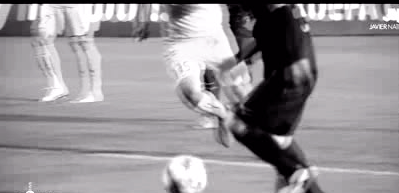
\includegraphics[scale=1]{imagenes/art1.png}

\subsection{Interpolación por Splines}

\begin{itemize}
\item Con seguridad, este hasta ahora es el método que genera los videos más fluidos.
\item Los movimientos de las cosas parecen naturales y no hay congelamientos ni transformaciones bruscas.
\item Esto se lo atribuimos a que el método en sí aprovecha todos los datos del pixel a tráves del tiempo para producir resultados mejores que tienen que ver con el marco teórico que le dan los polinomio interpoladores de Lagrange.
\item Eso si, siguen habiendo imágenes falsas a causa del movimiento y no son menores pero si ligeramente mejores que en la interpolación lineal.
\item Por ejemplo, en la instancia \textbf{skate}, los resultados son del estilo:
\end{itemize}

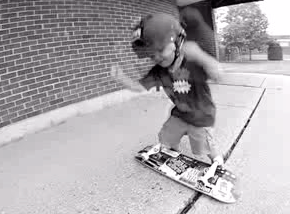
\includegraphics[scale=1]{imagenes/art2.png}

\subsection{Interpolación por Splines de a bloques de 4 pixeles}

\begin{itemize}
\item En este caso parece haber un retroceso de calidad con respecto al método anterior.
\item Los movimientos de las cosas parecen naturales.
\item Pero si hay congelamientos.
\item En particular, en el video \textbf{Messi} se nota claramente como la pelota se congela en algunos momentos.
\item Esto era de esperarse debido a los bloques de tamaño fijo ubicados a través del tiempo.
\end{itemize}


\newpage
\section{Conclusión}
%\setlength{\parindent}{15.0pt} % algún comando dejó en cero el parindent
En este trabajo pudimos no solo modelar el problema planteado, sino 
apreciar y aprovechar las propiedades del mismo para así resolverlo con los
métodos estudiados observando también las características de ellos.

Así mismo, cabe destacar que al realizar operaciones con aritmética finita,
tanto para la solución de los sistemas como para los valores evaluados en cada
interpolador, no podemos garantizar que los resultados obtenidos sean exactos,
pero dado que realizamos varias instancias de prueba con distintas metodologías,
pudimos ver que los valores que obtuvimos eran coherentes a su contexto.

Todos los métodos de interpolación realizados en este trabajo cumplieron con la
tarea de generar en mayor o menor medida el efecto de cámara lenta que
buscábamos cada uno con sus características particulares. Mediante la
experimentación pusimos bajo la lupa cada interpolador utilizado para así poder
compararlos entre sí.

Comenzamos nuestros experimentos probando el correcto funcionamiento de los
métodos implementados. Aquí además de ver mediante las cotas de precisión que
todos los métodos cumplían la tarea de interpolar las funciones predeterminadas
pudimos tener una primera visión sobre cómo se comportaba cada interpolador. El
más básico, por vecinos, efectivamente demostró tener la mayor cota de error
distanciándose ampliamente del resto, mientras que la interpolación lineal
obtuvo resultados similares a los obtenidos con splines. En este experimento en
particular, la interpolación mediante splines probó ser la de menor error,
superando a la lineal para funciones cuadráticas y cúbicas, donde a su vez se
pudo observar su relación con la interpolación por splines de a bloques, que con
bloques más grandes su cota se aproximaba a la del spline standard.

En la siguiente prueba, donde lo que se analizó fue el error producido al
elminar cuadros del video original e intentar recrearlos con nuestros
interpoladores, los resultados fueron similares al experimento anterior. Con
ambas fórmulas de cálculo de error (ECM y PSNR) se pudo ver cómo vecinos era el
método que peor se comportaba mientras que lineal y splines estuvieron
emparejados a lo largo de todas las instancias de prueba realizadas.

Finalmente, la búsqueda de artifacts en el video producido, de anomalías y
calidad final a nivel visual para el usuario resultó ser el punto determinante
para decidir cuál de los sistemas propuestos mejor se desempeña en la tarea de
proveer un efecto de cámara lenta. Los resultados acá dieron un giro completo
con respecto a las conclusiones que veníamos realizando respecto a las métricas
estudiadas. Para empezar, la interpolación de a vecinos dio mejores
resultados que la lineal en términos de cantidad de artifacts y calidad general
del video producido. El método por splines fue el que mejor llegó a producir la
sensación de cámara lenta, con algunas anomalías pero no lo suficientemente
signigicantes como las vistas en la interpolación lineal. Esto creemos que se
podría explicar con el hecho de que las métricas seleccionadas para decidir qué
interpolador era mejor estaban demasiado atadas a que interpolaran
correctamente sin contemplar cómo resultaba visualmente esta interpolación.

Por último, podemos mencionar como posibles desarrollos a futuro la búsqueda de
métricas que se centren más en el aspecto visual de los interpoladores,
distintas formas de interpolación o directamente métodos completamente
distintos, como lo sería considerar la aplicación de cuadrados mínimos, para
seguir comparando y buscando que se generen los menores artifacts posibles.


\newpage
%\bibliographystyle{plain}
\section{Referencias}
%\begingroup
%\renewcommand{\section}[2]{}
%\bibliography{informe}
%\endgroup

\newpage
\section{Enunciado}
%\noindent\textbf{Contexto y motivaci\'on}
\vskip 5pt

 
%\vskip 5pt
%\noindent\textbf{Contexto}
%\vskip 5pt

A partir de la evoluci\'on de Internet durante la d\'ecada de 1990, el desarrollo de motores de b\'usqueda se ha convertido en uno de los aspectos 
centrales para su efectiva utilizaci\'on. Hoy en d\'ia, sitios como Yahoo, Google y Bing ofrecen distintas alternativas para realizar b\'usquedas 
complejas dentro de un red que contiene miles de millones de p\'aginas web. 

En sus comienzos, una de las caracter\'isticas que distingui\'o a Google respecto de los motores de b\'usqueda de la \'epoca fue la calidad de los 
resultados obtenidos, mostrando al usuario p\'aginas relevantes a la b\'usqueda realizada. El esquema general de los or\'igenes de este motor de 
b\'usqueda es brevemente explicado en Brin y Page \cite{Brin1998}, donde se mencionan aspectos t\'ecnicos que van desde la etapa de obtenci\'on de
informaci\'on de las p\'aginas disponibles en la red, su almacenamiento e indexado y su posterior procesamiento, buscando ordenar cada p\'agina de 
acuerdo a su importancia relativa dentro de la red. El algoritmo utilizado para esta \'ultima etapa es denominado PageRank y es uno (no el \'unico) 
de los criterios utilizados para ponderar la importancia de los resultados de una b\'usqueda. En este trabajo nos concentraremos en el estudio y 
desarrollo del algoritmo PageRank.

Por otro lado, las competencias deportivas, en todas sus variantes y disciplinas, requieren casi inevitablemente la comparaci\'on entre competidores
mediante la confecci\'on de \emph{Tablas de Posiciones} y \emph{Rankings} en base a resultados obtenidos en un per\'iodo de tiempo determinado. 
Estos ordenamientos de equipos est\'an generalmente (aunque no siempre) basados en reglas relativamente claras y simples, como proporci\'on 
de victorias sobre partidos jugados o el cl\'asico sistema de puntajes por partidos ganados, empatados y perdidos. Sin embargo, estos m\'etodos
simples y conocidos por todos muchas veces no logran capturar la complejidad de la competencia y la comparaci\'on. Esto es particularmente
evidente en ligas donde, por ejemplo, todos los equipos no juegan la misma cantidad de veces entre s\'i.

A modo de ejemplo, la NBA y NFL representan dos ligas con fixtures de temporadas regulares con estas caracter\'isticas. Recientemente, el Torneo de 
Primera Divisi\'on de AFA se suma a este tipo de competencias, ya que la incorporaci\'on de la \emph{Fecha de Cl\'asicos} parece ser una interesante 
idea comercial, pero no tanto desde el punto de vista deportivo ya que cada equipo juega contra su \emph{cl\'asico} m\'as veces que el resto. 
Como contraparte, \'estos rankings son utilizados muchas veces como criterio de decisi\'on, como por ejemplo para determinar la participaci\'on en 
alguna competencia de nivel internacional, con lo cual la confecci\'on de los mismos constituye un elemento sensible, afectando intereses deportivos 
y econ\'omicos de gran relevancia.


\vskip 5pt
\noindent\textbf{El problema, Parte I: PageRank y p\'aginas web}
\vskip 5pt

El algoritmo PageRank se basa en la construcci\'on del siguiente modelo. Supongamos que tenemos una red con $n$ p\'aginas 
web $Web = \{1,\dots,n\}$ donde
el objetivo es asignar a cada una de ellas un puntaje que determine la importancia relativa de la misma respecto de las
dem\'as. Para modelar las relaciones entre ellas, definimos la \emph{matriz de conectividad} $W \in \{0,1\}^{n \times n}$ 
de forma tal que $w_{ij} = 1$ si la p\'agina $j$ tiene un link a la p\'agina $i$, y $w_{ij} = 0$ en caso contrario. 
Adem\'as, ignoramos los \emph{autolinks}, es decir, links de una p\'agina a s\'i misma, definiendo $w_{ii} = 0$. Tomando 
esta matriz, definimos el grado de la p\'agina $j$, $n_j$, como la cantidad de links salientes hacia otras p\'aginas 
de la red, donde $n_j = \sum_{i = 1}^n w_{ij}$. Adem\'as, notamos con $x_j$ al puntaje asignado a la p\'agina $j\in
Web$, que es lo que buscamos calcular.

La importancia de una p\'agina puede ser modelada de diferentes formas. Un link de la p\'agina $u \in
Web$ a la p\'agina $v \in Web$ puede ser visto como que $v$ es una p\'agina importante. Sin embargo, no queremos que una
p\'agina obtenga mayor importancia simplemente porque es apuntada desde muchas p\'aginas. 
Una forma de limitar esto es ponderar los links utilizando la importancia de la p\'agina de origen. En otras palabras,
pocos links de p\'aginas importantes pueden valer m\'as que muchos links de p\'aginas poco importantes. En particular,
consideramos que la importancia de la p\'agina $v$ obtenida mediante el link de la p\'agina $u$ es proporcional a la 
importancia de la p\'agina $u$ e inversamente proporcional al grado de $u$. Si la p\'agina $u$ contiene $n_u$ links,
uno de los cuales apunta a la p\'agina $v$, entonces el aporte de ese link a la p\'agina $v$ ser\'a $x_u/n_u$. Luego,
sea $L_k \subseteq Web$ el conjunto de p\'aginas que tienen un link a la p\'agina $k$. Para cada p\'agina pedimos que
\begin{eqnarray}
x_k = \sum_{j \in L_k} \frac{x_j}{n_j},~~~~k = 1,\dots,n. \label{eq:basicmodel}
\end{eqnarray}
Definimos $P \in  \mathbb{R}^{n \times n}$ tal que $p_{ij} = 1/n_j$ si $w_{ij} = 1$, y $p_{ij} = 0$ en caso contrario. Luego,
el modelo planteado en (\ref{eq:basicmodel}) es equivalente a encontrar un $x\in \mathbb{R}^n$ tal que $Px = x$, es
decir, encontrar (suponiendo que existe) un autovector asociado al autovalor 1 de una matriz cuadrada, tal que $x_i \ge
0$ y $\sum_{i = 1}^n x_i = 1$. En
Bryan y Leise \cite{Bryan2006} y Kamvar et al. \cite[Secci\'on 1]{Kamvar2003} se analizan ciertas condiciones que debe
cumplir la red de p\'aginas para garantizar la existencia de este autovector.

Una interpretaci\'on equivalente para el problema es considerar al \emph{navegante aleatorio}. \'Este empieza en una
p\'agina cualquiera del conjunto, y luego en cada p\'agina $j$ que visita sigue navegando a trav\'es de sus links,
eligiendo el mismo con probabilidad $1/n_j$. Una situaci\'on particular se da cuando la p\'agina no tiene links salientes. En
ese caso, consideramos que el navegante aleatorio pasa a cualquiera de las p\'agina de la red con probabilidad $1/n$.
Para representar esta situaci\'on, definimos $v \in \mathbb{R}^{n \times n}$, con $v_i = 1/n$ y $d \in \{0,1\}^{n}$ donde 
$d_i = 1$ si $n_i = 0$, y $d_i = 0$ en caso contrario. La nueva matriz de transici\'on es 
\begin{eqnarray*}
D & = & v d^t \\
P_1 & = & P + D.
\end{eqnarray*}
Adem\'as, consideraremos el caso de que el navegante aleatorio, dado que se encuentra en la p\'agina $j$, decida visitar
una p\'agina cualquiera del conjunto, independientemente de si esta se encuentra o no referenciada por $j$ (fen\'omeno
conocido como \emph{teletransportaci\'on}). Para ello, consideramos que esta decisi\'on se toma con una probabilidad
$c \ge 0$, y podemos incluirlo al modelo de la siguiente forma:
\begin{eqnarray*}
E & = & v \bar{1}^t \\
P_2 & = & cP_1 + (1-c)E,
\end{eqnarray*}
\noindent donde $\bar{1} \in \mathbb{R}^n$ es un vector tal que todas sus componentes valen 1. La matriz resultante
$P_2$ corresponde a un enriquecimiento del modelo formulado en (\ref{eq:basicmodel}). Probabil\'isticamente, la
componente $x_j$ del vector soluci\'on (normalizado) del sistema $P_2 x = x$ representa la proporci\'on del tiempo que,
en el largo plazo, el navegante aleatorio pasa en la p\'agina $j \in Web$. Denotaremos con $\pi$ al vector soluci\'on 
de la ecuaci\'on $P_2 x = x$, que es com\'unmente denominado \emph{estado estacionario}.

En particular, $P_2$ corresponde a una
matriz \emph{estoc\'astica por columnas} que cumple las hip\'otesis planteadas en Bryan y Leise \cite{Bryan2006} y
Kamvar et al. \cite{Kamvar2003}, tal que $P_2$ tiene un autovector asociado al autovalor 1, los dem\'as autovalores de
la matriz cumplen $1 = \lambda_1 > |\lambda_2| \ge \dots \ge |\lambda_n|$ y, adem\'as, la dimensi\'on
del autoespacio asociado al autovalor $\lambda_1$ es 1. Luego, $\pi$ puede ser calculada
de forma est\'andar utilizando el m\'etodo de la potencia.

Una vez calculado el ranking, se retorna al usuario las $t$ p\'aginas con mayor puntaje.

\vskip 5pt
\noindent\textbf{El problema, Parte II: PageRank y ligas deportivas}
\vskip 5pt

Existen en la literatura distintos enfoques para abordar el problema de determinar el \emph{ranking} de equipos de una competencia en
base a los resultados de un conjunto de partidos. En Govan et al. \cite{Govan2008} se hace una breve rese\~na de dos ellos, y los autores
proponen un nuevo m\'etodo basado en el algoritmo PageRank que denominan GeM\footnote{Aunque no se especifica, asumimos que el nombre se
debe a las iniciales de los autores.}. Conceptualmente, el m\'etodo GeM representa la temporada como un red (grafo) donde las p\'aginas web
representan a los equipos, y existe un link (que tiene un valor, llamado peso, asociado) entre dos equipos que los relaciona modelando los resultados de los posibles
enfrentamientos entre ellos. En base a este modelo, Govan et al. \cite{Govan2008} proponen calcular el ranking de la misma forma que en el 
caso de las p\'aginas web.

En su versi\'on b\'asica, que es la que consideraremos en el presente trabajo, el m\'etodo GeM (ver, e.g., \cite[Secci\'on GeM Ranking Method]{Govan2008}) 
es el siguiente\footnote{Notar que en art\'iculo, Govan et al. \cite{Govan2008} lo definen sobre la traspuesta. La definici\'on y las cuentas son
equivalentes, simplemente se modifica para mantener la consistencia a lo largo del enunciado.}:
\begin{enumerate}
\item La temporada se representa mediante un grafo donde cada equipo representa un nodo y existe un link de $i$ a $j$ si el equipo $i$ perdi\'o al
menos una vez con el equipo $j$.
\item Se define la matriz $A^t \in \mathbb{R}^{n \times n}$

\begin{equation*}
A_{ji}^t = \left\{
	\begin{array}{cl}
	w_{ji} & \text{si el equipo } i \text{ perdi\'o con el equipo } j,\\
	0 & \text{en caso contrario, }\\
	\end{array} \right.
\end{equation*}

\noindent donde $w_{ji}$ es la diferencia absoluta en el marcador. En caso de que $i$ pierda m\'as de una vez con $j$, $w_{ji}$ representa la suma
acumulada de diferencias. Notar que $A^t$ es una generalizaci\'on de la matriz de conectividad $W$ definida en la secci\'on anterior.

\item Definir la matriz $H_{ji}^t \in \mathbb{R}^{n \times n}$ como
\begin{equation*}
H_{ji}^t = \left\{
	\begin{array}{cl}
	A_{ji}^t/\sum_{k = 1}^n A_{ki}^t & \text{si hay un link } i \text{ a } j,\\
	0 & \text{en caso contrario.}\\
	\end{array} \right.
\end{equation*}

\item Tomar $P = H^t$, y aplicar el m\'etodo PageRank como fue definido previamente, siendo $\pi$ la soluci\'on a la ecuaci\'on $P_2 x = x$. Notar que 
los p\'aginas sin links salientes, en este contexto se corresponden con aquellos equipos que se encuentran invictos.

\item Utilizar los puntajes obtenidos en $\pi$ para ordenar los equipos.
\end{enumerate}

En funci\'on del contexto planteado previamente, el m\'etodo GeM define una estructura que relaciona equipos dependiendo de los resultados parciales y
obtener un ranking utilizando solamente esta informaci\'on.

\vskip 5pt
\noindent\textbf{Enunciado}
\vskip 5pt

El objetivo del trabajo es experimentar en el contexto planteado utilizando el algoritmo PageRank con las variantes propuestas. A su vez, se busca
comparar los resultados obtenidos cualitativa y cuantitativamente con los algoritmos tradicionales utilizados en cada uno de los contextos planteados. 
Los m\'etodos a implementar (como m\'inimo) en ambos contexto planteados por el trabajo son los siguientes:

\begin{enumerate}
\item \emph{B\'usqueda de p\'aginas web:} PageRank e \textsc{In-deg}, \'este \'ultimo consiste en definir el ranking de las p\'aginas utilizando 
solamente la cantidad de ejes entrantes a cada una de ellas, orden\'andolos en forma decreciente.
\item \emph{Rankings en competencias deportivas:} GeM y al menos un m\'etodo est\'andar propuesto por el grupo (ordenar por victorias/derrotas,
puntaje por ganado/empatado/perdido, etc.) en funci\'on del deporte(s) considerado(s).
\end{enumerate}

El contexto considerado en 1., en la b\'usqueda de p\'aginas web, representa un desaf\'io no s\'olo desde el modelado, si no tambi\'en desde el punto 
de vista computacional considerando la dimensi\'on de la informaci\'on y los datos a procesar. Luego, dentro de nuestras posibilidades, consideramos
un entorno que simule el contexto real de aplicaci\'on donde se abordan  instancias de gran escala (es decir, $n$, el n\'umero total de p\'aginas, es 
grande). Para el desarrollo de PageRank, se pide entonces considerar el trabajo de Bryan y Leise \cite{Bryan2006} donde se explica la intuci\'on y algunos 
detalles t\'ecnicos respecto a PageRank. Adem\'as, en Kamvar et al. \cite{Kamvar2003} se propone una mejora del mismo. Si bien esta mejora queda fuera de 
los alcances del trabajo, en la Secci\'on 1 se presenta una buena formulaci\'on del algoritmo. En base a su definici\'on, $P_2$ no es una matriz esparsa. 
Sin embargo, en Kamvar et al. \cite[Algoritmo 1]{Kamvar2003} se propone una forma alternativa para computar $x^{(k+1)} = P_2 x^{(k)}$. Este resultado debe 
ser utilizado para mejorar el almacenamiento de los datos.

En la pr\'actica, el grafo que representa la red de p\'aginas suele ser esparso, es decir, una p\'agina posee relativamente pocos links de salida comparada 
con el n\'umero total de p\'aginas. A su vez, dado que $n$ tiende a ser un n\'umero muy grande, es importante tener en cuenta este hecho a la hora de definir 
las estructuras de datos a utilizar. Luego, desde el punto de vista de implementaci\'on se pide utilizar alguna de las siguientes estructuras de datos para 
la representaci\'on de las matrices esparsas: \emph{Dictionary of Keys} (dok), \emph{Compressed Sparse Row} (CSR) o \emph{Compressed Sparse Column} (CSC). 
Se deber\'a incluir una justificaci\'on respecto a la elecci\'on que consdiere el contexto de aplicaci\'on. Adem\'as, para PageRank se debe implementar el 
m\'etodo de la potencia para calcular el autovector principal. Esta implementaci\'on debe ser realizada \'integramente en \textsc{C++}.

En funci\'on de la experimentaci\'on, se deber\'a realizar un estudio particular para cada algoritmo (tanto en t\'erminos de comportamiento
del mismo, como una evaluaci\'on de los resultados obtenidos) y luego se proceder\'a a comparar cualitativamente los rankings generados.
La experimentaci\'on deber\'a incluir como m\'inimo los siguientes experimentos:
\begin{enumerate}
\item Estudiar la convergencia de PageRank, analizando la evoluci\'on de la norma Manhattan (norma $L_1$) entre dos iteraciones sucesivas. Comparar los 
resultados obtenidos para al menos dos instancias de tama\~no mediano-grande, variando el valor de $c$. 
\item Estudiar el tiempo de c\'omputo requerido por PageRank. 
\item Para cada algoritmo, proponer ejemplos de tama\~no peque\~no que ilustren el comportamiento esperado (puede ser utilizando las herramientas provistas
por la c\'atedra o bien generadas por el grupo).
\end{enumerate}

Puntos opcionales:
\begin{enumerate}
\item Demostrar que los pasos del Algoritmo 1 propuesto en Kamvar et al. \cite{Kamvar2003} son correctos y computan $P_2 x$.
\item Establecer una relaci\'on con la proporci\'on entre $\lambda_1 = 1$ y $|\lambda_2|$ para la convergencia de PageRank.
\end{enumerate}

El segundo contexto de aplicaci\'on no presenta mayores desaf\'ios desde la perspectiva computacional, ya que en el peor de los casos una liga no suele tener
mas que unas pocas decenas de equipos. M\'as a\'un, es de esperar que en general la matriz que se obtiene no sea esparsa, ya que probablemente un equipo juegue
contra un n\'umero significativo de contrincantes. Sin embargo, la popularidad y sensibilidad del problema planteado requieren de un estudio detallado y 
pormenorizado de la calidad de los resultados obtenidos. El objetivo en este segundo caso de estudio es puramente experimental. 

En funci\'on de la implementaci\'on, a\'un cuando no represente la mejor opci\'on, es posible reutilizar y adaptar el desarrollo realizado para p\'aginas web. 
Tambi\'en es posible realizar una nueva implementaci\'on desde cero, simplificando la operatoria y las estructuras, en \textsc{C++}, \textsc{Matlab} o 
\textsc{Python}.

La experimentaci\'on debe ser realizada con cuidado, analizando (y, eventualmente, modificando) el modelo de GeM:
\begin{enumerate}
\item Considerar al menos un conjunto de datos reales, con los resultados de cada fecha para alguna liga de algu\'un deporte.
\item Notar que el m\'etodo GeM asume que no se producen empates entre los equipos (o que si se producen, son poco frecuentes). En caso de considerar un 
deporte donde el empate se da con cierta frecuencia no despreciable (por ejemplo, f\'utbol), es fundamental aclarar como se refleja esto en el modelo y 
analizar su eventual impacto.
\item Realizar experimentos variando el par\'ametro $c$, indicando como impacta en los resultados. Analizar la evoluci\'on del ranking de los equipos a 
trav\'es del tiempo, evaluando tambi\'en la evoluci\'on de los rankings e identificar caracter\'isticas/hechos particulares que puedan ser determinantes 
para el modelo, si es que existe alguno.
\item Comparar los resultados obtenidos con los reales de la liga utilizando el sistema est\'andar para la misma.
\end{enumerate}

Puntos opcionales:
\begin{enumerate}
\item Proponer (al menos) dos formas alternativas de modelar el empate entre equipos en GeM.
\end{enumerate}


\vskip 5pt
\noindent\textbf{Par\'ametros y formato de archivos}
\vskip 5pt

El programa deber\'a tomar por l\'inea de comandos dos par\'ametros. El primero de ellos contendr\'a la informaci\'on del experimento, incluyendo
el m\'etodo a ejecutar (\verb+alg+, 0 para PageRank, 1 para el m\'etodo alternativo), la probabilidad de teletransportaci\'on $c$, el tipo de instancia
(0 p\'aginas web, 1 deportes), el \emph{path} al archivo/directorio conteniendo la definici\'on de la red (que debe ser relativa al ejecutable, o el path 
absoluto al archivo) y el valor de tolerancia utilizado en el criterio de parada del m\'etodo de la potencia. 

El siguiente ejemplo muestra un caso donde se pide ejecutar PageRank, con una probabilidad de teletransportaci\'on de 0.85, sobre la red descripta en 
\verb+test1.txt+ (que se encuentra en el directorio \verb+tests/+), correspondiente a una instancia de ranking aplicado a deportes y con una tolerancia 
de corte de $0.0001$.
\begin{verbatim}
0 0.85 1 tests/red-1.txt 0.0001
\end{verbatim}

Para la definici\'on del grafo que representa la red, se consideran dos bases de datos de instancias con sus correspondientes formatos. La primera
de ellas es el conjunto provisto en SNAP \cite{SNAP} (el tipo de instancia es 0), con redes de tama\~no grande obtenidos a partir de datos reales. Adem\'as, 
se consideran las instancias que se forman a partir de resultados de partidos entre equipos, para alg\'un deporte elegido por el grupo. 

En el caso de la base de SNAP, los archivos contiene primero cuatro l\'ineas con informaci\'on sobre la instancia (entre ellas, $n$ y la cantidad
total de links, $m$) y luego $m$ l\'ineas con los pares $i$, $j$ indicando que $i$ apunta a $j$. A modo de ejemplo, a continuaci\'on se muestra el 
archivo de entrada correspondiente a la red propuesta en Bryan y Leise \cite[Figura 1]{Bryan2006}: 

\begin{verbatim}
# Directed graph (each unordered pair of nodes is saved once): 
# Example shown in Bryan and Leise.
# Nodes: 4 Edges: 8 
# FromNodeId    ToNodeId
1   2
1   3
1   4
2   3
2   4
3   1
4   1
4   3
\end{verbatim}

Para el caso de rankings en ligas deportivas, el archivo contiene primero una l\'inea con informaci\'on sobre la cantidad de equipos ($n$), y la cantidad
de partidos totales a considerar ($k$). Luego, siguen $k$ l\'neas donde cada una de ellas representa un partido y contiene la siguiente informaci\'on: 
n\'umero de fecha (es un dato opcional al problema, pero que puede ayudar a la hora de experimentar), equipo $i$, goles equipo $i$, equipo $j$, goles equipo $j$.
A continuaci\'on se muestra el archivo de entrada con la informaci\'on del ejemplo utilizado en Govan et al. \cite{Govan2008}:

\begin{verbatim}
6 10
1 1 16 4 13
1 2 38 5 17
1 2 28 6 23
1 3 34 1 21
1 3 23 4 10
1 4 31 1 6
1 5 33 6 25
1 5 38 4 23
1 6 27 2 6
1 6 20 5 12
\end{verbatim}

Es importante destacar que, en este \'ultimo caso, los equipos son identificados mediante un n\'umero. Opcionalmente podr\'a considerarse un archivo que contenga, 
para cada equipo, cu\'al es el c\'odigo con el que se lo identifica.

Una vez ejecutado el algoritmo, el programa deber\'a generar un archivo de salida que contenga una l\'inea por cada
p\'agina ($n$ l\'ineas en total), acompa\~nada del puntaje obtenido por el algoritmo PageRank/\textsc{In-deg}/m\'etodo alternativo. 

Para generar instancias de p\'aginas web, es posible utilizar el c\'odigo Python provisto por la c\'atedra. La utilizaci\'on del mismo se
encuentra descripta en el archivo README. Es importante mencionar que, para que el mismo funcione, es
necesario tener acceso a Internet. En caso de encontrar un bug en el mismo, por favor contactar a los docentes de la
materia a trav\'es de la lista. Desde ya, el c\'odigo puede ser modificado por los respectivos grupos agregando todas
aquellas funcionalidades que consideren necesarias.

Para instancias correspondientes a resultados entre equipos, la c\'atedra provee un conjunto de archivos con los resultados del Torneo de Primera Divisi\'on 
del F\'utbol Argentino hasta la Fecha 23. Es importante aclarar que los dos partidos suspendidos, River - Defensa y Justicia y Racing - Godoy Cruz han sido 
arbitrariamente completados con un resultado inventado, para simplificar la instancia. En funci\'on de datos reales, una alternativa es considerar el 
repositorio DataHub \cite{datahub}, que contiene informaci\'on estad\'istica y resultados para distintas ligas y deportes de todo el mundo.

\vskip 5pt

\hrule

\vskip 5pt


{\bf \underline{Fechas de entrega}}
\begin{itemize}
 \item \emph{Formato Electr\'onico:} Martes 6 de Octubre de 2015, hasta las 23:59 hs, enviando el trabajo (informe +
 c\'odigo) a la direcci\'on \verb+metnum.lab@gmail.com+. El subject del email debe comenzar con el texto \verb+[TP2]+
 seguido de la lista de apellidos  de los integrantes del grupo.
 \item \emph{Formato f\'isico:} Mi\'ercoles 7 de Octubre de 2015, a las 18 hs. en la clase pr\'actica.
\end{itemize}

\noindent \textbf{Importante:} El horario es estricto. Los correos recibidos despu\'es de la hora indicada ser\'an considerados re-entrega.  




\newpage
\appendix
%%\newpage
\section{Código C++} \label{sec:codigo}

\newcommand{\codelst}{\begingroup
  \catcode`_=12 \docodelst}
\newcommand{\docodelst}[1]{%
  \lstinputlisting[language=C++]{#1}%
  \endgroup
}

\subsection*{video.cpp}
\codelst{../src/video.cpp}
\subsection*{interpolador.h}
\codelst{../src/interpolador.h}
\subsection*{spline.cpp}
\codelst{../src/spline.cpp}
\subsection*{lineal.h}
\codelst{../src/lineal.cpp}
\subsection*{vecinos.cpp}
\codelst{../src/vecinos.cpp}
\subsection*{multi_spline.cpp}
\codelst{../src/multi_spline.cpp}
\subsection*{test_utils.h}
\codelst{../src/test_utils.h}


\end{document}
